\chapter{Big Picture}% by Saad Bin Quddus}

\begin{linkb}
   \begin{itemize}
        \item \href{https://www.youtube.com/watch?v=7x3lxFRwi6Y}{Big picture (Saad)}
        \item \href{https://drive.google.com/file/d/1g92Ymk1uX2tE9Xu4hYwaIncj5K_g3kYR/view}{Zhao}
   \end{itemize}
\end{linkb}

(This class is taught by following Yufei Zhao's \textit{Cyclic Quadrilateral: The Big Picture Note}.)
Here Saad vai started with Spiral Similarity. A very common trick in Olympiad Geometry. Then  he went to the Miquels theorem for Triangle and Quadrilateral.




\section{Spiral Similarity}
What is a spiral similarity. It is a special type of similarity which arise anturally. Spiral Similarity is a rotation with a dilation or homothety centered at a single point. 

\begin{lemma}
Let $AB$ and $CD$ be segments, and suppose $X = AC \cap BD$. If $(ABX)$ and $(CDX)$ intersect again at $O$, then $O$ is the center of the unique spiral
similarity taking $AB$ into $CD$.
\end{lemma}


\begin{figure}[ht]
\centering
	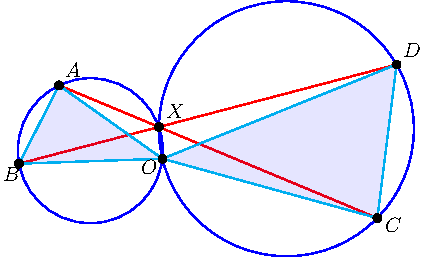
\includegraphics{spiral-lemma.pdf}
	\caption{Spiral Similarity Lemma}
\end{figure}

You may wonder that spiral similarity comes in pairs. As the next proposition says:
\begin{proposition}
The center of spiral similarity takin $AB$ to $CD$ is also the center of the spiral similarity taking $AC$ to $BD$.
\end{proposition}


\section{Miquel's Theorem}


\begin{theorem}[Miquel's Theorem]
Let $ABC$ be a triangle and $D,E,F$ eb the points on $BC,CA,AB$ respectively. Then the circumcircles of the triangles $AEF, BDF, CDE$ are concurrent.
\end{theorem}
\begin{figure}[ht]
\centering
	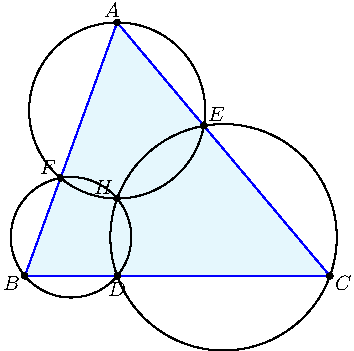
\includegraphics{miq-tri.pdf}
	\caption{Miquel's Theorem on $\triangle ABC$.}
\end{figure}
\begin{proof}
Let $(BDF) \cap (CDE)=H$.
Here we angle chase:
\[\angle EHF=\angle B +\angle C = 180 -\angle A.\]
done!
Another aproah is :
\[\angle AFH = \angle HDB, \angle AEH =\angle HDC.\]
which sum to $180\dg$.
\end{proof}
Note that $D,E,F$ can lie on the extension of the segments.


Here we are going to the Miquel's Quadrilateral Theorem which arise naturally.

\begin{theorem}[Miquel's (Quadrilateral) Theorem]
The four circles $(PAB), (PDC), (QAD), (QBC)$
concur at the Miquel point $M$. Furthermore, 
$M$ is the center of the spiral similarity sending
$AB$ to $DC$ and $BC$ to $AD$. (In particular,
 $ \triangle MAB \sim \triangle MDC$ and $\triangle MBC \sim \triangle MAD.$)
\end{theorem}
\begin{figure}[ht]
\centering
	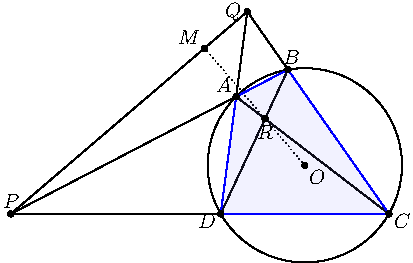
\includegraphics{miq-quad.pdf}
	\caption{Miquel's Theorem in Complete Quadrilateral.}
\end{figure}
The above theorem is same as the theorem for triangle's. Just consider thriangle $QDC$ and $P,A,B$ on the corresponding segments!

\begin{proof}
Let $M$ be the second intersection between $(QAB)$ and $(QCD)$ and by spiral similarity, $M$ is the center of the spiral similarity taking $AB$ to $CD$. SO, it is also the center of spiral similarity taking $BC$ to $DA$. By converse direction of the lemma $M$ lies on $(PAD)$ and $(ABC)$.
\end{proof}

Now we are going to see some properties of Miquel Point of a cyclic quadrilaral. It is known that \textit{One of the most powerful configurations in olympiad geometry is the Miquel point when
complete quadrilateral ABCD is cyclic}.

\begin{theorem}[Miquel's Theorem on a Cyclic Quadrilateral]
Miquel's Point has more properties in a cyclic quadrilateral. Beacuse of the fact that, $M$ is the inverse of $R$ (intersection of the diagonals) with respect to inversion around $(ABCD)$. 
\begin{itemize}
	\ii %$M$ is the common point of 
	The six circles $(OAC), (OBD), (P AD)$, $(P BC), (QAB),(QCD)$ goes through a single point i.e. $M$.
	\ii $M$ is the center of a spiral similarity taking $AB$ to $CD$, as well as the spiral similarity taking $BC$ to $DA$.
	\ii $M$ is the inverse of $R = AC \cap BD$ with respect to an inversion around $(ABCD)$. By Brocard’s theorem, $M$ is the foot of $O$ onto $PQ$.
	\ii $OM\perp PQ$.
\end{itemize}
\end{theorem}
These results also can be proved by angle chasing as well as spiral similarity. 

%\section{}









